\documentclass[11pt, letterpaper, includehead]{article}

%%%%%%%%%%%%%%%%%%%%% Pre-document %%%%%%%%%%%%%%%%%%%%%
\usepackage{fancyhdr}  % Allow for headers
\usepackage{graphicx}  % Allow for figures 
\usepackage{float}     % Allow for figure inserted in specified location
\usepackage{amsmath}   % Allow for aligned math
\usepackage{array}     % Allow for cell width manipulation
\usepackage{nicematrix}
\usepackage{amssymb} % Uhhhh what was this????
\usepackage{multicol}

\setlength{\parindent}{0pt} % Remove auto paragraph indents

% Get rid of those big ass margins
\usepackage[margin=1in]{geometry}

% Table cell formatting
\setlength{\arrayrulewidth}{0.25mm}
\setlength{\tabcolsep}{11pt}
\renewcommand{\arraystretch}{1.2}

\begin{document}

%%%%%%%%%%%%%%%%%%%%% Title Page %%%%%%%%%%%%%%%%%%%%%
\begin{titlepage}
  \begin{center}
    \Huge{\textbf{Lab 7}}\\
    \Huge{Work and Mechanical Energy}
    \vfill
    \begin{figure}[H] % H makes the figure insert at the position in the document
      \centering 
      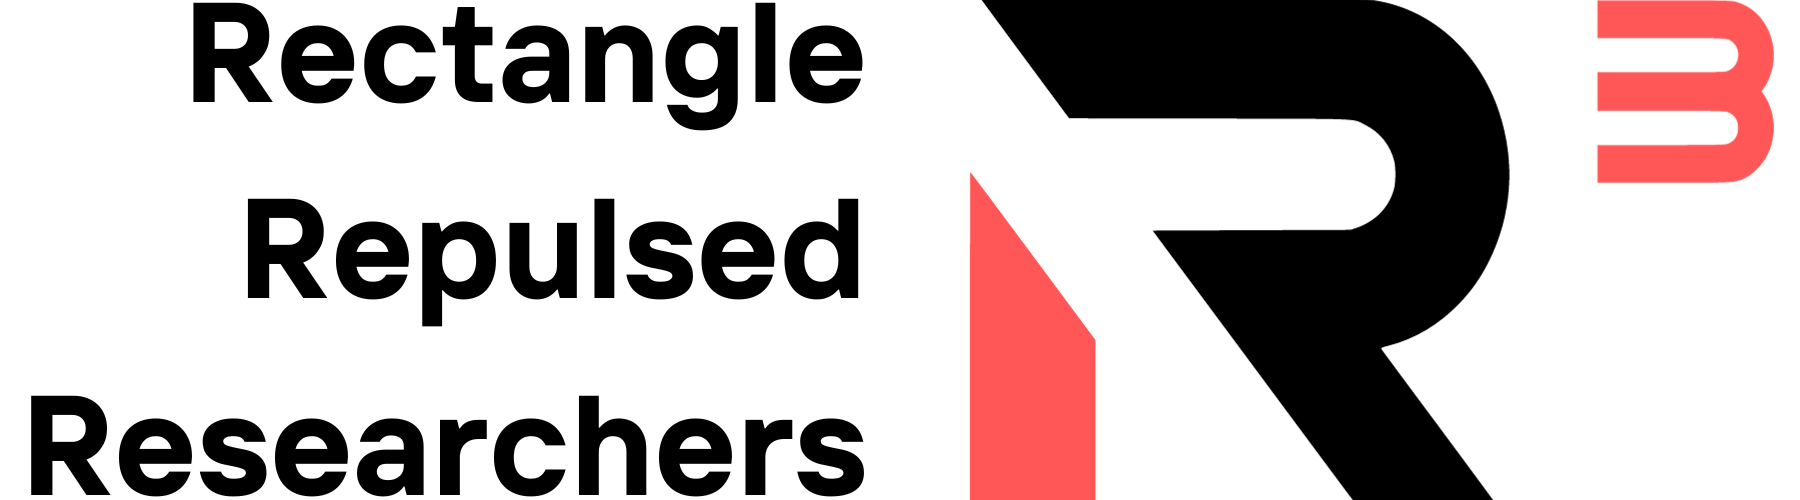
\includegraphics[width=6cm]{../logo.png}
    \end{figure}
    \large{\textbf{your name here}}\\
    \large{Julian Barossi, Liam Gilligan, Stephanie L'Heureux}\\
    \vspace{0.5cm}
    \normalsize
    \today
  \end{center}
\end{titlepage}

%%%%%%%%%%%%%%%%%%%%% TABLE OF CONTENTS %%%%%%%%%%%%%%%%%%%%%
\tableofcontents
\pagebreak % Move to next page

% Add a nice fancy header
\pagestyle{fancy}
\fancyhead{}
\fancyhead[C]{\textbf{Lab 7:} Work and Mechanical Energy}

\section{Trial 1} % 1
\subsection{Data}
\begin{center} 
  \begin{tabular}{|m{1.8cm}|m{1.8cm}|m{2.2cm}|m{2.5cm}|m{3cm}|} 
    \hline
    \boldmath{$m_{cart}\,(kg)$} & \boldmath{$\Delta{x}\,(m)$} & \boldmath{$m_{weight}\, (kg)$} & \boldmath{\textbf{Tension} $(N)$} & \boldmath{\textbf{Velocity} $(m/s)$}\\ 
       \hline
       0.256 & 0.5 & 0.02 & 0.17465 & 0.77365 \\
       \hline
  \end{tabular} 
\end{center}
\subsection{Measured Kinetic Energy}
Using the mass and speed of the cart, we can find it's kinetic energy using
the equation below.\\\\
$$K_f = \frac{1}{2}m\cdot v^2$$
$$K_f = \frac{1}{2}0.256kg\cdot (0.77365m/s)^2$$
$$K_f \approx 0.07661J$$\\

\subsection{Work Done by Tension}
By taking our measured tension and multiplying it by the displacement,
we can get the work $(W_{ext})$ done on the cart.

$$W_{ext} = \vec{F}\cdot \vec{r}$$
$$W_{ext} = |F||r|\cos\theta$$
$$W_{ext} = (0.17465N)(0.500m)\cos0^{\circ}$$
$$W_{ext} = (0.17465N)(0.500m)$$
$$W_{ext} \approx 0.08733J$$\\

\subsection{Percent Difference Between Kinetic Energy and Work}
$$\Delta K = K_f + K_i = K_f$$

$$\%diff = \frac{|A - B|}{(A + B) / 2}\cdot 100\%$$
$$\%diff = \frac{|W_{ext} - \Delta K|}{(W_{ext} + \Delta K) / 2}\cdot 100\%$$
$$\%diff = \frac{|0.08733J - 0.07661J|}{(0.08733J + 0.07661J) / 2}\cdot 100\%$$\\
$$\%diff \approx \boxed{13.0691437\%}$$\\

\subsection{Calculate Theoretical Tension and Compare to Measured}
$$T_{thy} = \frac{m_{cart}\cdot m_{weight}\cdot g}{m_{cart} + m_{weight}}$$
$$T_{thy} = \frac{0.256kg\cdot 0.02kg\cdot 9.80m/s^2}{0.256kg + 0.02kg}$$
$$T_{thy} = 0.1817971014N \approx \boxed{0.182N}$$\\

$$\%diff = \frac{T_{exp} - T_{thy}}{T_{thy}}\cdot 100\%$$
$$\%diff = \frac{0.175N - 0.182N}{0.182N?.}\cdot 100\%$$
$$\%diff \approx \boxed{-3.931361607\%}$$

\section{Trial 2} % 2
\subsection{Data}
\begin{center} 
  \begin{tabular}{|m{1.8cm}|m{1.8cm}|m{2.2cm}|m{2.5cm}|m{3cm}|} 
    \hline
    \boldmath{$m_{cart}\,(kg)$} & \boldmath{$\Delta{x}\,(m)$} & \boldmath{$m_{weight}\, (kg)$} & \boldmath{\textbf{Tension} $(N)$} & \boldmath{\textbf{Velocity} $(m/s)$}\\ 
       \hline
       0.256 & 0.5 & 0.03 & 0.24241 & 0.9507 \\
       \hline
  \end{tabular} 
\end{center}
\subsection{Measured Kinetic Energy}
Using the mass and speed of the cart, we can find it's kinetic energy using
the equation below.\\\\
$$K_f = \frac{1}{2}m\cdot v^2$$
$$K_f = \frac{1}{2}0.256kg\cdot (0.9507m/s)^2$$
$$K_f \approx 0.1157J$$\\

\subsection{Work Done by Tension}
By taking our measured tension and multiplying it by the displacement,
we can get the work $(W_{ext})$ done on the cart.

$$W_{ext} = \vec{F}\cdot \vec{r}$$
$$W_{ext} = |F||r|\cos\theta$$
$$W_{ext} = (0.24241N)(0.500m)\cos0^{\circ}$$
$$W_{ext} = 0.1212J$$
$$W_{ext} \approx 0.1212J$$\\

\subsection{Percent Difference Between Kinetic Energy and Work}
$$\Delta K = K_f + K_i = K_f$$

$$\%diff = \frac{|A - B|}{(A + B) / 2}\cdot 100\%$$
$$\%diff = \frac{|W_{ext} - \Delta K|}{(W_{ext} + \Delta K) / 2}\cdot 100\%$$
$$\%diff = \frac{|0.1212J - 0.1157J|}{(0.1212J + 0.1157J) / 2}\cdot 100\%$$\\
$$\%diff \approx \boxed{4.655809733\%}$$\\

\subsection{Calculate Theoretical Tension and Compare to Measured}
$$T_{thy} = \frac{m_{cart}\cdot m_{weight}\cdot g}{m_{cart} + m_{weight}}$$
$$T_{thy} = \frac{0.256kg\cdot 0.03kg\cdot 9.80m/s^2}{0.256kg + 0.03kg}$$
$$T_{thy} = 0.2631608392N \approx \boxed{0.2632N}$$\\

$$\%diff = \frac{T_{exp} - T_{thy}}{T_{thy}}\cdot 100\%$$
$$\%diff = \frac{0.2424N - 0.2632N}{0.2632N}\cdot 100\%$$
$$\%diff \approx \boxed{-3.931361607\%}$$

\section{Trial 3} % 1
\subsection{Data}
\begin{center} 
  \begin{tabular}{|m{1.8cm}|m{1.8cm}|m{2.2cm}|m{2.5cm}|m{3cm}|} 
    \hline
    \boldmath{$m_{cart}\,(kg)$} & \boldmath{$\Delta{x}\,(m)$} & \boldmath{$m_{weight}\, (kg)$} & \boldmath{\textbf{Tension} $(N)$} & \boldmath{\textbf{Velocity} $(m/s)$}\\ 
       \hline
       0.256 & 0.5 & 0.04 & 0.3192 & 1.0655 \\
       \hline
  \end{tabular} 
\end{center}
\subsection{Measured Kinetic Energy}
Using the mass and speed of the cart, we can find it's kinetic energy using
the equation below.\\
$$K_f = \frac{1}{2}m\cdot v^2$$
$$K_f = \frac{1}{2}0.256kg\cdot (1.0655m/s)^2$$
$$K_f \approx \boxed{0.1453J}$$\\

\subsection{Work Done by Tension}
By taking our measured tension and multiplying it by the displacement,
we can get the work $(W_{ext})$ done on the cart.

$$W_{ext} = \vec{F}\cdot \vec{r}$$
$$W_{ext} = |F||r|\cos\theta$$
$$W_{ext} = (0.3192N)(0.500m)\cos0^{\circ}$$
$$W_{ext} = \boxed{0.1596J}$$

\subsection{Percent Difference Between Kinetic Energy and Work}
$$\Delta K = K_f + K_i = K_f$$

$$\%diff = \frac{|A - B|}{(A + B) / 2}\cdot 100\%$$
$$\%diff = \frac{|W_{ext} - \Delta K|}{(W_{ext} + \Delta K) / 2}\cdot 100\%$$
$$\%diff = \frac{|0.1596J - 0.1453J|}{(0.1596J + 0.1453J) / 2}\cdot 100\%$$\\
$$\%diff \approx \boxed{9.368346717\%}$$\\

\subsection{Calculate Theoretical Tension and Compare to Measured}
$$T_{thy} = \frac{m_{cart}\cdot m_{weight}\cdot g}{m_{cart} + m_{weight}}$$
$$T_{thy} = \frac{0.256kg\cdot 0.04kg\cdot 9.80m/s^2}{0.256kg + 0.04kg}$$
$$T_{thy} = 0.2631608392N \approx \boxed{0.3390N}$$\\

$$\%diff = \frac{T_{exp} - T_{thy}}{T_{thy}}\cdot 100\%$$
$$\%diff = \frac{0.3192N - 0.3390N}{0.3390N}\cdot 100\%$$
$$\%diff \approx \boxed{-5.848214286\%}$$

\section{Analysis}
\subsection{Why don't we need to include the work done by other forces?}
The only other forces acting on the system are perpindicular
to the motion of the system, therefore meaning the work would be zero
since the $\theta$ between the motions and the force is $90^{\circ}$.
\subsection{Why is the total energy of the system only equal to the kinetic energy of the cart?}
There is no change in height, so there is no change in gravitational potential
energy, there is no spring in the system so there is no spring potential energy.
There is, however, some amount of heat generated, or $\Delta E_{th}$ as there is friction,
but we do not consider this as the friction is significantly low.

\end{document}